
The Hidden Markov Model (HMM) is one of the most common sequence
probabilistic models, and has been applied to a wide variety of
tasks. More generally, an HMM is a particular instance of  a chain
directed probabilistic graphical model, or a Bayesian network.  In a
Bayesian network, every random variable is represented as a node in a
graph, and the edges in the graph are directed and represent
probabilistic dependencies between the random variables. For an HMM, the random variables are divided into two sets, the 
\emph{observed} variables, in our case 
$\obs$, and the \emph{hidden} variables, in our case $\hs$. In the HMM
terminology, the observed variables are called \emph{observations}, and the
hidden variables are called \emph{states}. 

As you may find out in today's lab session, 
implementing the inference routines of the HMM can be challenging, 
and debugging can become hard in large
datasets. We thus start with a small and very
simple (very unrealistic!) example. The idea is that you may compute the desired
quantities by hand and check if your implementation yields the correct result. 

\begin{example}

Consider a person, which is only interested in four activities: 
\begin{itemize}
\item walking in
the park (w);
\item shopping (s);
\item cleaning his apartment (c);
\item playing tennis (t).
\end{itemize}
The choice of what to do on a given day is determined exclusively by the weather at that day. The
weather can be either \emph{rainy} (r) or \emph{sunny} (s). 
Now, suppose that we observe what the person did on a sequence of days; 
can we use that information to predict the weather each of those days? 
To tackle this problem, we assume 
that the weather behaves as a discrete Markov Chain: the weather on a
given day is independent of everything else \emph{given 
the weather on the previous day}. The entire system is that of a hidden Markov model (HMM).

Assume we are asked to predict what was the weather on two different
sequences of days given the following observations: ``walk walk shop
clean''  and ``clean walk tennis walk ''. This will be our test set.


To train our model, we will be given access to three different sequences of
days, containing both the activities and the weather on those days, namely: 
``walk/rainy walk/sunny shop/sunny
clean/sunny'', ``walk/rainy walk/rainy shop/rainy clean/sunny '' and ``walk/sunny shop/sunny shop/sunny clean/sunny''. This
will be our training set.
 \end{example}

It is useful to artificially introduce a special ``STOP'' state at the end of the sequence, which marks its end. This is useful for two reasons: it simplifies the notation, and it also allows our model to cope with sequences of any finite size (otherwise, how would our model cope with natural sentences, which can range from one or two words to dozens?).

Figure \ref{hmm} shows the HMM model for the first sequence of our simple
example, already including the ``STOP'' symbol. The notation is summarized in Table \ref{tab:hmm-simple-notation}. Note that $i,j$ can go up to $N+1$ due to the ``STOP'' symbol.


\begin{table}[h]
\begin{center}
\begin{tabular}{|l|l|}
\hline
\multicolumn{2}{|c|}{HMM Example}\\
\hline
\hline
$\sent$ & observed sentence ``w w s c'' \\
\hline
$N = 4$ & observation length \\
\hline
$i,j$ & positions in the sentence: $i,j \in \{1 \ldots N\}$ \\
\hline
$\vocab = \{w,s,c,t\}$ & observation vocabulary \\
\hline 
$p,q$ & indexes into the vocabulary $p,q \in |\vocab|$\\
\hline
$\obs_i = \vv_q,\obs_j = \vv_p$ & observation at position $\obs_i$ ($\obs_j$) has value $\vv_q$ ($\vv_p$)\\
\hline 
$\hvocab = \{r,s\}$ & hidden values vocabulary\\
\hline 
$l,m$ & indexes into the hidden values vocabulary\\
\hline
$\hs_i = \hv_l,\hs_j = \hv_m$ & state at position $\hs_i$ ($\hs_j$) has hidden value $\hv_l$ ($\hv_m$)\\
\hline
\end{tabular}
\end{center}
\caption[HMM notation]{\label{tab:hmm-simple-notation} HMM notation for the running example.}
\end{table}

\begin{figure}[ht]
\centering
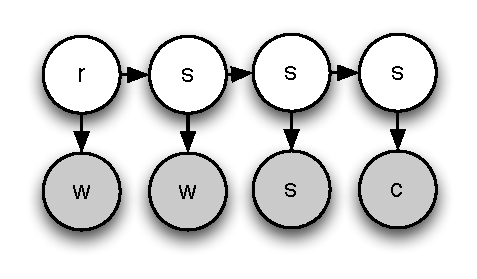
\includegraphics[width=0.6\textwidth]{figs/sequences/hmm}
\caption[HMM running example]{\label{fig:hmm} HMM structure, for the simple
running example.}
\end{figure}


A first order HMM model has the following independence assumptions over the joint distribution $\joint$:
\begin{itemize}
  \item \textbf{Independence of previous states.} The probability of
    being in a given state $\hv_l$ at position $\hs_i$ only depends on
    the state $\hv_m$ of the previous position $\hs_{i-1}$. Formally, 
    $p_{\theta} (\hs_i = \hv_l \mid \hs_{i-1} = \hv_m, \hs_{i-2} \ldots \hs_{1}) = p_{\theta} (\hs_i = \hv_l \mid \hs_{i-1} = \hv_m)$, 
    defining a first order Markov chain.%
    \footnote{The order of the Markov chain depends on the number of previous positions taken into account. 
    The remainder of the exposition can be easily extended to higher order HMMs, giving the model more generality, 
    but making inference harder.}
  \item \textbf{Homogeneous transition.} The probability of
    making a transition from state $\hv_l$ to state $\hv_m$ is independent of
    the particular position in the sentence: for all $i,j \in \{1,\ldots,N\}$,
    $p_{\theta} (\hs_i = \hv_l \mid \hs_{i-1} = \hv_m) =  p_{\theta}
    (\hs_j = \hv_l \mid \hs_{j-1} = \hv_m)$, so
    $p_{\theta} (\hs_i = \hv_l \mid \hs_{i-1} = \hv_m) = p_{\theta} (\hv_l \mid \hv_m)$.
  \item \textbf{Observation independence.}  The probability of
    observing $\vv_q$ at position $i$ is fully determined by the state
    at that position. Formally, $p_{\theta} (\obs_i = \vv_q \mid \hs_i = \hv_l, \hs_{i-1}, \hs_{i-2} \ldots \hs_{1}) = p_{\theta}(\obs_i = \vv_q\mid
    \hs_i=\hv_l)$, and this probability is independent of the
    particular position, that is  $p_{\theta}(\obs_i = \vv_q\mid
    \hs_i=\hv_l)  = p_{\theta}(\vv_q\mid \hv_l)$.
\end{itemize}
These conditional independence assumptions are crucial to allow
efficient inference, as will be described.

We also need to define a \emph{start probability}, the probability of starting 
at state $\hv_l$.
%Furthermore, when dealing with text, it is usual to break the homogeneous transition for the last position, and model the final transitions as independent parameters.
 The three probability
distributions that define the HMM model are summarized in Table
\ref{tab:hmm-dist}. 
For each one
of them we will use a short notation to simplify the exposition.
\begin{table}[h]
\begin{center}
\begin{tabular}{|l|l|l|}
\hline
\multicolumn{3}{|c|}{HMM distributions}\\
\hline
Name & probability distribution & short notation \\
\hline
\textbf{initial probability} & $p_{\theta} (\hs_1 = \hv_l)$ & $\pi_{l}$\\
\hline
%\textbf{final probability} & $p_{\theta} (\hs_T = \hv_l \mid
%\hs_{T-1} = \hv_m)$ & $f_{m,l}$\\
%\hline
\textbf{transition probability} & $p_{\theta} (\hs_i = \hv_l \mid
\hs_{i-1} = \hv_m)$ & $a_{m,l}$\\
\hline
\textbf{observation probability} & $p_{\theta}(\obs_i = \vv_q\mid \hs_i = \hv_l)$ & $b_l(\obs_i) $ \\
\hline
\end{tabular}
\end{center}
\caption[HMM probability distributions]{\label{tab:hmm-dist} HMM probability distributions.}
\end{table}

The joint distribution can be expressed as:
\begin{equation}
  \joint =\pi_{\hs_1}b_{\hs_1}(\obs_1) [\prod_{i=2}^{N}
  a_{\hs_{i-1},\hs_{i}} b_{\hs_{i}}(\obs_i)] a_{\hs_{i},STOP},
  \label{eqn:hmm}
\end{equation}
which for the example from Figure \ref{fig:hmm} is:
\begin{equation}
  \joint =\pi_{r} b_r("w") a_{r,s}b_s("w") a_{s,s}b_s("s") a_{s,s}b_s("c")a_{s,STOP}.
  \label{eqn:hmm_ex}
\end{equation}
%
Here is a detailed explanation of the terms:
\begin{equation}
  \joint = \hspace{-1.5cm}\underbrace{\pi_{r}}_{\text{prob. of starting at state ``r''}} \hspace{-2cm}\overbrace{b_r("w")}^{\text{prob. of observing ``w'' if state is ``r''}} \hspace{-2cm}\underbrace{a_{r,s}}_{\text{prob. of going from state ``r'' to state ``s''}} \hspace{-2cm}\overbrace{b_s("w")}^{\text{prob. of observing ``w'' if state is ``s''}} \hspace{-1cm}\underbrace{a_{s,s}b_s("s") a_{s,s}b_s("c")}_{\text{etc...}} \hspace{-1.5cm}\overbrace{a_{s,STOP}}^{\text{prob. of going from state ``s'' to state ``STOP''}}
%  \label{eqn:hmm_ex}
\end{equation}

\begin{exercise}
Load the simple sequence dataset:
From the ipython command line (Note: start ipython from the \emph{lxmls}
directory), create a simple sequence object and look at the training
and test set.
\begin{python}
 In[]: run readers/simple_sequence.py
 In[]: simple = SimpleSequence()
 In[]: simple.train
Out[]: [w/r w/s s/s c/s , w/r w/r s/r c/s , w/s s/s s/s c/s ]
 In[]: simple.test
Out[]: [w/r w/s s/s c/s , c/s w/s t/s w/s ] 
\end{python}
\end{exercise}
%%% Local Variables: 
%%% mode: latex
%%% TeX-master: "../../guide"
%%% End: 


%There is one problem left to solve. How do we know when the sequence ends? In the above example, the model would continue to generate states and symbols forever, but our training and test sets have finite sentences. Furthermore, in many applications sentences are not all of the same length, as happens with natural text. To cope with this, one usually adds a special ``STOP'' symbol which denotes the end of the sequence. Then, the sequence ``w w s c'' becomes ``w/r w/s s/s c/s STOP/STOP'', the set of states goes from \{``s'',``r''\} to \{``s'',``r'',``STOP''\}


In the next section we turn our attention to estimating the different
probability distributions of the model: $\pi_l$, $a_{m,l}$ and $b_l(\obs_i)$.
